\section{Validation du cahier des charges} 
La mise en oeuvre des algorithmes et programmes décrits précédemment nous à permis d'aboutir à un jeu fonctionnel, simple et respectant le cahier des charges.

\subsection{Le Plateau}

Comme nous l'avions envisagé, nous avons décidé d'utiliser un fond d'écran différent pour chaque état de jeu en respectant les dimensions imposées. Par soucis d'homogénéité, nous avons choisi un ensemble d'images sur le thème "épouvante".
\begin{figure}[H]
   \begin{minipage}[c]{.46\linewidth}
      
\includegraphics[scale=0.3]{img/backgroundaccueil.png}
			 \caption {Ecran d'accueil} 
   \end{minipage} \hfil
   \begin{minipage}[c]{.46\linewidth}
      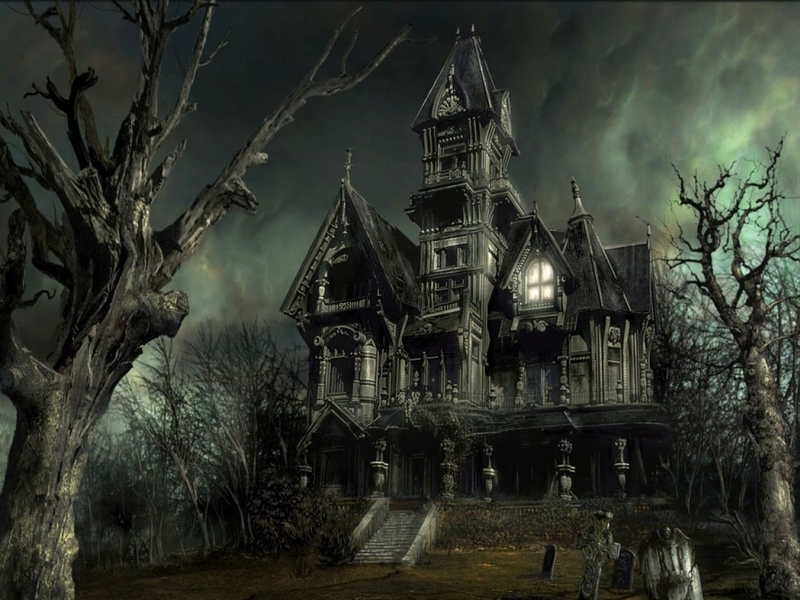
\includegraphics[scale=0.83]{img/maison.jpg}
			\caption {Menu} 
   \end{minipage}
\end{figure}
\begin{figure}[H]
   \begin{minipage}[c]{.46\linewidth}
      
\includegraphics[scale=0.3]{img/livre.jpg}
			\caption {Ecran des Scores} 
   \end{minipage} \hfil
   \begin{minipage}[c]{.46\linewidth}
      
\includegraphics[scale=0.3]{img/option.jpg}
			\caption {Ecran d'options} 
   \end{minipage}
\end{figure}
\begin{figure}[H]
   \begin{minipage}[c]{.46\linewidth}
      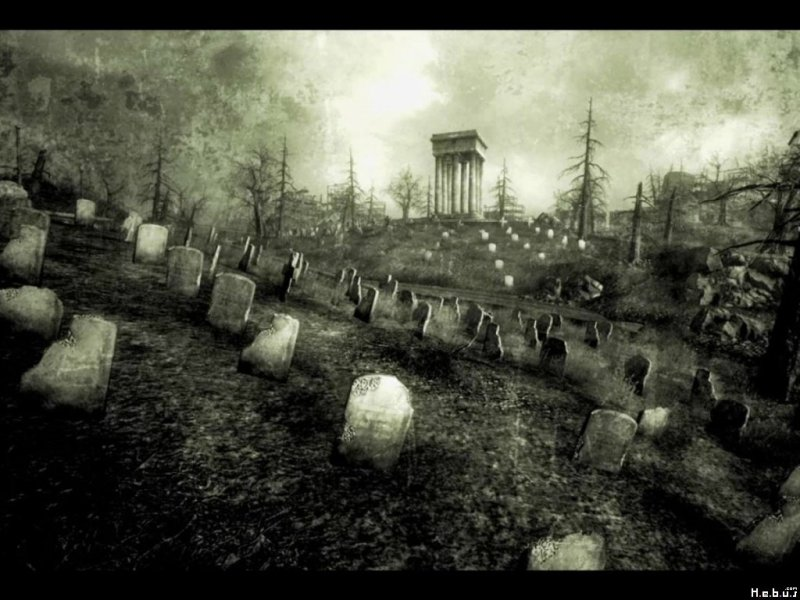
\includegraphics[scale=0.3]{img/background.jpg}
			\caption {Ecran de jeu} 
   \end{minipage} \hfil
   \begin{minipage}[c]{.46\linewidth}
      
\includegraphics[scale=0.3]{img/backgroundover.jpg}
			\caption {Ecran de défaite} 
   \end{minipage}
\end{figure}

C'est donc avec ces images que nous avons créer nos fonds d'écran.


\subsection{L'Accueil}

Cet écran placé avant le menu invite le joueur a écrire son prénom de manière à l'enregegistrer pour la comptabilité des scores.
\begin{figure}[H]
   \begin{minipage}[c]{.46\linewidth}
      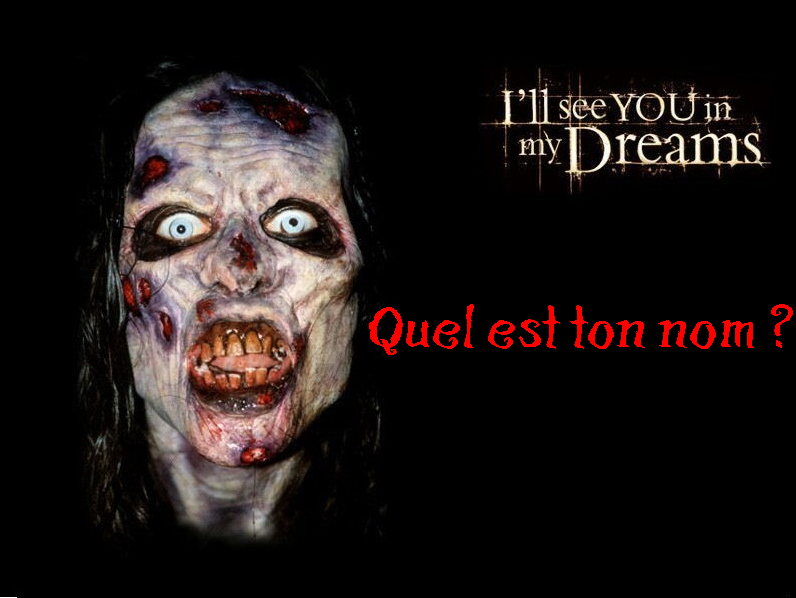
\includegraphics[scale=0.3]{img/accueilquestion.png}
			 \caption {question posée au joueur} 
   \end{minipage} \hfil
   \begin{minipage}[c]{.46\linewidth}
      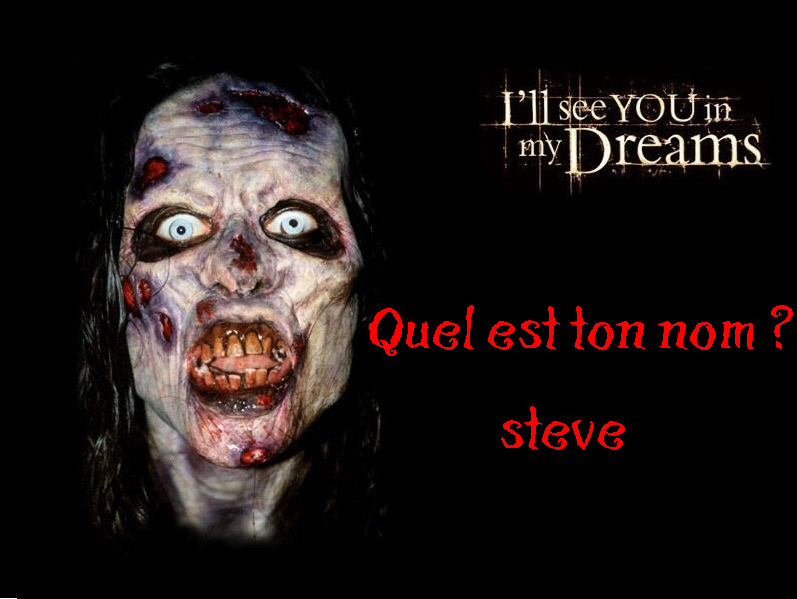
\includegraphics[scale=0.3]{img/accueilnom.png}
			\caption {Le joueur écrit son nom} 
   \end{minipage}
\end{figure}

\subsection{Le Menu}
Nous avons choisi un menu assez sobre affichant le nom du joueur et lui laissant la possiblité de quitter le jeu.
\begin{figure}[H]
\begin{center}
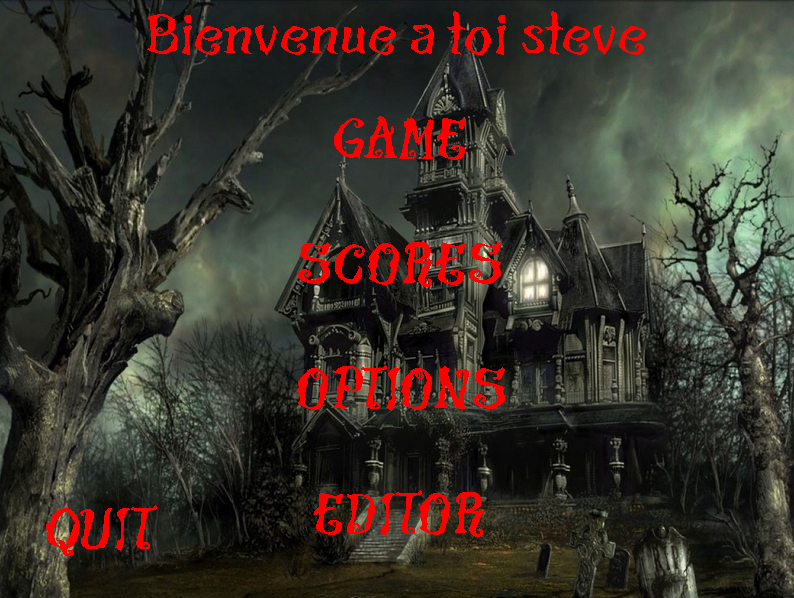
\includegraphics[scale=0.3]{img/menucomplet.png}
\caption {Ecran de menu}
\end{center}
\end{figure}
Il propose des liens vers le jeu, les scores, les options et l'éditeur de niveau au moyen d'un click.


\subsection{Les Niveaux}

Les deux niveaux fournis représentent une spirale et un parcours en zigzag. L'éditeur que nous avons créé présente la forme suivante.
\begin{figure}[H]
   \begin{minipage}[c]{.46\linewidth}
      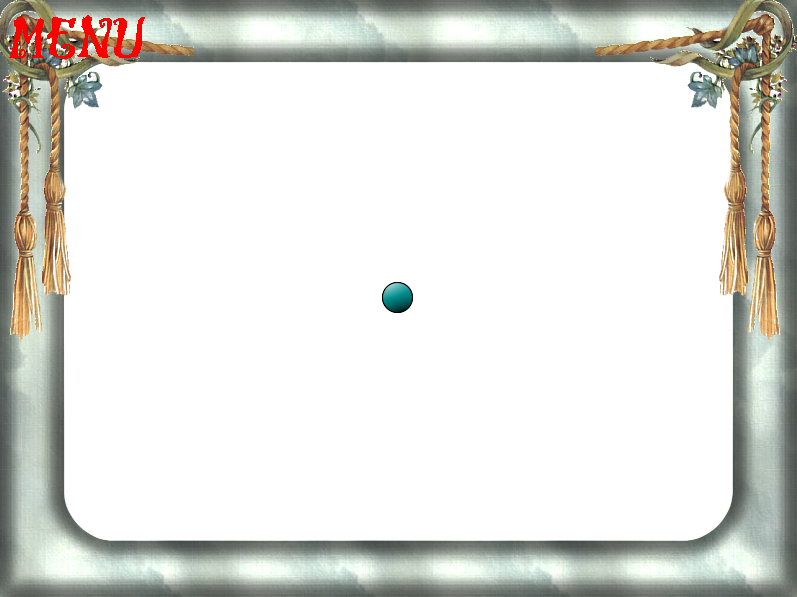
\includegraphics[scale=0.3]{img/editor.png}
			\caption {Editeur avant le tracé} 
   \end{minipage} \hfil
   \begin{minipage}[c]{.46\linewidth}
      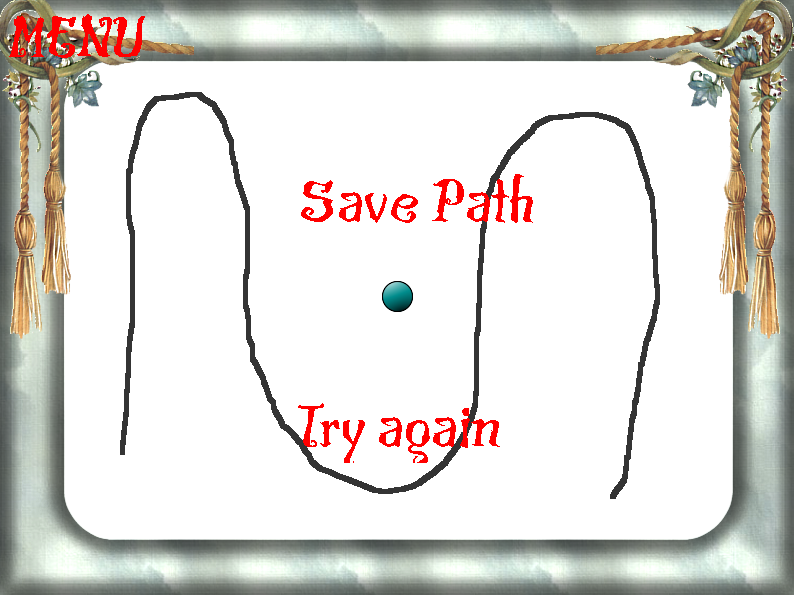
\includegraphics[scale=0.3]{img/editorpath.png}
			\caption {Tracé effectué} 
   \end{minipage}
\end{figure}
\begin{figure}[H]
\begin{center}
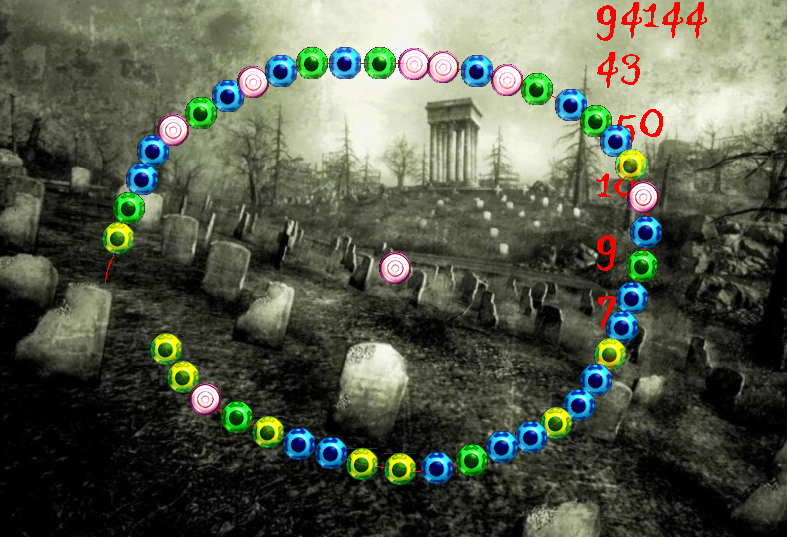
\includegraphics[scale=0.4]{img/bonparcours.png}
\caption {Exemple de parcours créé avec l'éditeur}
\end{center}
\end{figure}
La boule symbolise le canon pour que le joueur n'effectue pas de tracé dessus.Le tracé commence au premier click gauche et dure jusqu'au relâchement de celui-ci De plus, un point de doit apparaître qu'une seul fois. Une fois le tracé effectué, l'algorithme relie les points trop éloignés et le joueur à la possibilité entre recommencer ou enregistrer. Dans ce dernier cas un fichier .txt du même format que les autres parcours est créé et le joueur n'a plus qu'à le renommer avec un numéro et le placer dans le dossier "level".


\subsection{Les Scores}

Les scores sont comptabilisés pour une partie et une difficulté donnée. Lors d'une partie, un score est attribué à chaque fois qu'il y a une collision, le score final étant la somme de ses scores temporaires :
$$Score=150(N_{boules}-2)$$ 
Il est possible de visionner l'historiques des scores en cliquant sur les flèches "haut" et "bas". Pour visionner les scores d'une autre difficulté, il suffit de cliquer sur les flèches "gauche" et "droite".
\begin{figure}[H]
\begin{center}
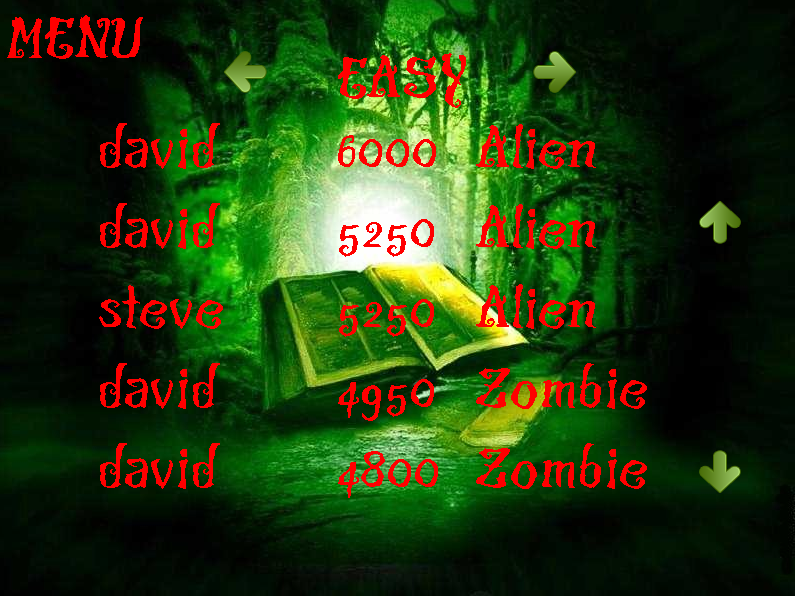
\includegraphics[scale=0.3]{img/scor.png}
\caption {Ecran des scores}
\end{center}
\end{figure}
 Suivant le score, un rang est attribué au joueur comme suit :
\begin{itemize}
  \item plus de 5000 : Alien 
  \item entre 3000 et 5000 : Zombie 
  \item entre 1000 et 3000 : Mutant
  \item moins de 1000 : Fantôme
\end{itemize} 

\subsection{Les Options}

L'écran d'option gère la présence du son, le thème des boules ainsi que la difficulté.
\begin{figure}[H]
\begin{center}
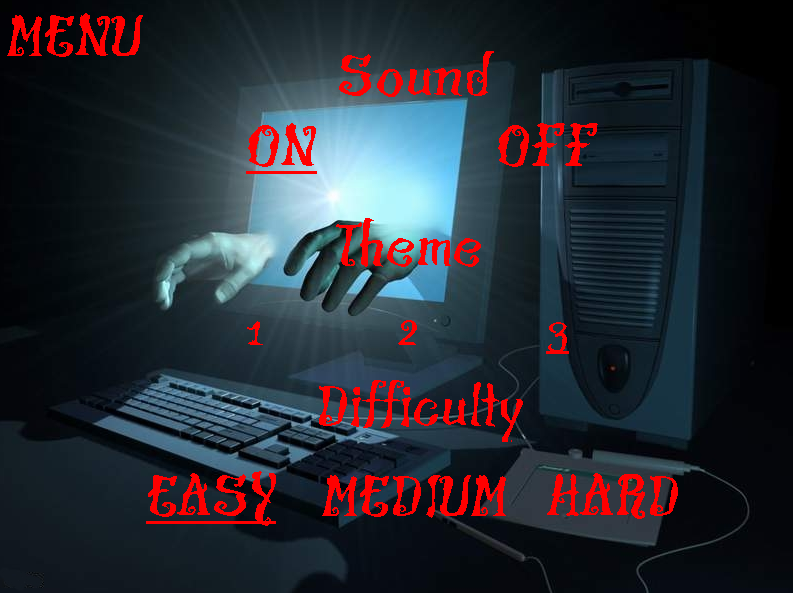
\includegraphics[scale=0.3]{img/optionscomplet.png}
\caption {L'Ecran des options}
\end{center}
\end{figure}
L'affichage de cet écran entraine le chargement du fichier option. Les options enregistrées sont soulignées. Un click sur une option entraine l'activation immédiate et la sauvegarde de celle-ci. Elle se souligne instantanément.

\subsection{Le Son}
Le son présent dans notre jeu est la bande originale du film "L'exorciste". Si le son est activé, la musique démarre dès l'écran d'accueil et continue pendant la navigation dans les menus mais s'arrête lors du jeu. Sinon, il est possible de l'activer dans l'écran d'option et la musique démarre alors. Malheureusement, il arrive que sur certaines machines, la gestions des sons en mp3 ne soit pas prise en charge. 

\subsection{Les Boules}

Comme nous souhaitions le faire, nous avons ajouter 2 types de boules utilisables par le joueur, l'un un rapport au thème de l'épouvante, l'autre constitué de boules colorées à l'aspect différent.
Voici les différentes boules utilisées :
\begin{figure}[H]
\begin{center}
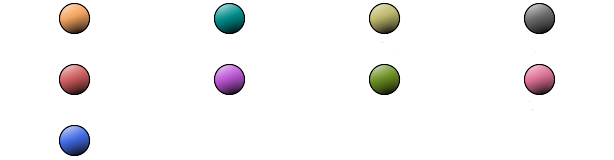
\includegraphics[scale=0.5]{img/boules1.png}
\caption {Boules fournies au début du BE}
~\\
~\\
~\\
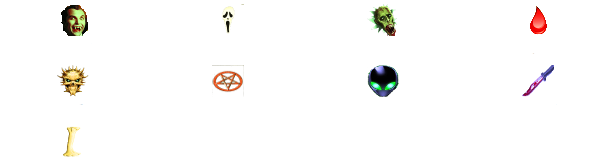
\includegraphics[scale=0.5]{img/boules2.png}
\caption {Boules en accord avec le thème du jeu}
~\\
~\\
~\\
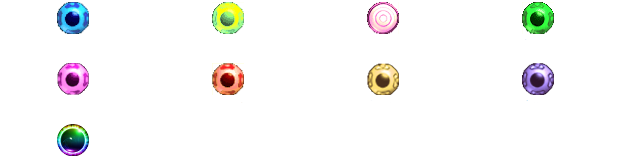
\includegraphics[scale=0.5]{img/boules3.png}
\caption {Boules colorées}
\end{center}
\end{figure}

\subsection{Les Difficultés}
Il est possible de choisir parmi 3 niveaux de difficulté, déterminés par des lois donnant le nombre de boules dans le cortège et le nombre de couleurs différentes :
$$N_{boules}=30+20(diff+1)$$
$$N_{couleurs}=2+2(diff+1)$$
Avec diff allant de 0(Easy) à 2(Hard). Soit :
\begin{itemize}
  \item Easy : 50 boules et 4 couleurs
  \item Medium : 70 boules et 6 couleurs
  \item Hard : 90 boules et 8 couleurs
\end{itemize} 
